\chapter{CVE-2025-21756}

\section{Overview}
CVE-2025-21756 is a use-after-free vulnerability identified in the Linux kernel's AF\_VSOCK subsystem, which is used for communication between hosts and virtual machines. The vulnerability allows a local attacker to gain elevated privileges (up to root) by exploiting incorrect management of the socket object lifecycle within the kernel.

The problem arises during specific sequences of operations on vsock sockets, leading to the dereferencing of memory structures that have already been freed and, consequently, to kernel memory corruption. Specifically, an attacker could exploit this vulnerability to achieve privilege escalation.

\section{The VSOCK subsystem}\label{vsock_subsystem}
VSOCK is a component of the Linux kernel that manages communication between a virtual machine (\textit{guest}) and the system hosting it (\textit{host}). It was developed in response to the need to provide a method of communication between the two entities that offers better performance than traditional network interfaces. Unlike TCP/IP sockets, which are based on IP addresses and network protocols, vsock sockets use an addressing model specific to virtualised environments. Communication via vsock utilises a pair of identifiers:
\begin{itemize}
    \item \textbf{CID (Context IDentifier)}: uniquely identifies an endpoint (host or VM)
    \item \textbf{Port}: similar to TCP/UDP ports
\end{itemize}
Some relevant CID values may include:
\begin{itemize}
    \item \texttt{VMADDR\_CID\_HOST}: represents the host
    \item \texttt{VMADDR\_CID\_LOCAL}: local communication
    \item specific CIDs assigned to individual VMs
\end{itemize}
The advantage of this model is that it avoids the overhead associated with the IP stack.\\
Communication takes place via two transport networks:
\begin{itemize}
    \item \textbf{G2H (guest-to-host)}: these are executed on the guest and are usually device drivers. We distinguish between three types:
    \begin{itemize}
        \item \textit{virtio-transport}: typical of KVM/QEMU, it uses virtqueues located within the guest as buffers, but the host also reads from and writes to them.

        \item \textit{vmci-transport}: VMWare's proprietary for H2G/G2H.

        \item \textit{hyperv-transport}: based on Hyper-V VMBus, designed specifically for Microsoft environments.
    \end{itemize}

    \item \textbf{H2G (host-to-guest)}: these are run on the host and usually provide device emulation for the guest. There are two types:
    \begin{itemize}
        \item \textit{vhost-transport}: host-side backend for virtio-transport.

        \item \textit{vmci-transport}: VMWare's proprietary for H2G/G2H.
    \end{itemize}
\end{itemize}
To illustrate communication between the host and the guest, we can use QEMU, an open-source emulator and virtualisation program, as an example. When creating a virtual machine, the structure will be as follows:
\begin{itemize}
    \item \textit{virtio-transport} on the guest
    \item \textit{vhost-transport} on the host: provides in-kernel device emulation to the guest and uses \texttt{ioeventfd} and \texttt{irqfd} to receive and send events to the guest.
\end{itemize}
\begin{figure}[h]
    \centering
    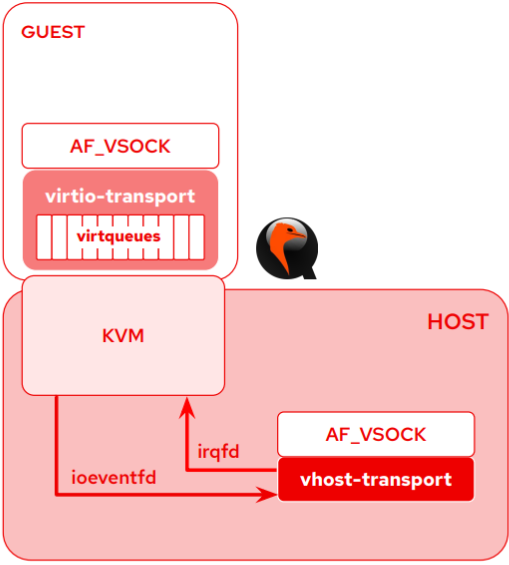
\includegraphics[scale=.4]{images/vsock.png}
    \caption{Example of a VSOCK communication structure.}
    \label{fig:vsock}
\end{figure}
Both provide an interface to the socket layer via the vsock core and exchange packets with virtio queues (\textit{virtqueues}).\\
KVM (Kernel-based Virtual Machine) turns the host OS into the VM's hypervisor, enabling it to manage the CPU and memory directly.

\subsubsection{Virtqueues}
These are shared buffer queues in memory that allow the two parties to communicate bidirectionally (even though a single virtqueue is dedicated to a single direction) while maintaining low overhead.\\
In \textbf{split virtqueue} mode (classic), they are based on three main shared memory areas:
\begin{itemize}
    \item \textbf{Descriptor Area}: contains the buffer metadata (the guest's physical address and length).

    \item \textbf{Available Ring}: a list of buffers that the driver has added and which are ready to be consumed by the host device.

    \item \textbf{Used Ring}: a list of buffers that the device has finished processing and is returning to the driver.
\end{itemize}
The \textbf{packed virtqueue} mode, on the other hand, uses a more modern and compact layout, merging the available and used rings, thereby improving the performance of the processor cache.\\
The operation can be broken down into the following stages:
\begin{enumerate}
    \item \textbf{Insertion}: the VirtIO (guest) driver places the buffers in the \textit{descriptor area} and updates the \textit{available ring}.

    \item \textbf{Notification (Kick)}: The driver sends a notification to the device ("doorbell") to indicate that new data is available.

    \item \textbf{Processing} of data by the host.

    \item \textbf{Completion}: the host updates the \textit{used ring} and sends an interrupt to the guest to signal completion.
\end{enumerate}
The virtqueue backend (which actually manages the queue on the host) can be \textbf{QEMU}, with full emulation, as in the case under consideration, or \textbf{vhost}: the backend runs within the host kernel (vhost-net/vhost-blk), allowing the driver to communicate directly with the kernel without going through QEMU's user space, thereby drastically reducing latency.

\subsubsection{Internal architecture of VSOCK}
From an implementation perspective, each vsock socket is represented in the kernel by a data structure (\texttt{struct vsock\_sock}), which extends the generic socket structures (\texttt{struct sock}). These objects are managed via:
\begin{itemize}
    \item \textbf{status lists}:
    \begin{itemize}
        \item \textit{bound sockets}: associated with a port;
        \item \textit{unbound sockets}: created but not yet associated;
    \end{itemize}
    \item \textbf{connection queue}: handling of incoming requests;
    \item \textbf{reference counting}: a fundamental mechanism for managing the life cycle of objects.
\end{itemize}
When consistency in the management of these elements is lacking, there is a risk of encountering the problems mentioned above, exposing the system to risks and attacks.

\subsubsection{The life cycle of a VSOCK socket}
Typically, a vsock socket goes through the following stages:
\begin{enumerate}
    \item \textbf{Creation} (\texttt{socket()}): memory is allocated for the data structure, which is then added to the \textit{unbound} list.

    \item \textbf{Binding} (\texttt{bind()} or autobind): the socket is associated with a port and is consequently added to the \textit{bound} list.

    \item \textbf{Connection} (\texttt{connect()} / \texttt{accept()}): the actual communication channel is established.

    \item \textbf{Release} (\texttt{close()}): when the socket is no longer needed, it is removed from the internal structures, its reference count is decremented and, if this reaches zero, its memory is deallocated.
\end{enumerate}

\section{Cause of the vulnerability}
The cause of CVE-2025-21756 may be considered trivial at the code level, but given that certain preconditions are required for the problem to occur, and given that the result is not readily apparent, identifying it was by no means straightforward.

% TODO - dettagli

\section{Test case presented by the developers}
Let's start with a test case provided by the maintainers of the VSOCK module for the Linux kernel, who, after releasing the patch, made it available to allow users to check whether their system is affected by the issue.
\clearpage
\begin{figure}[H]
    \centering
    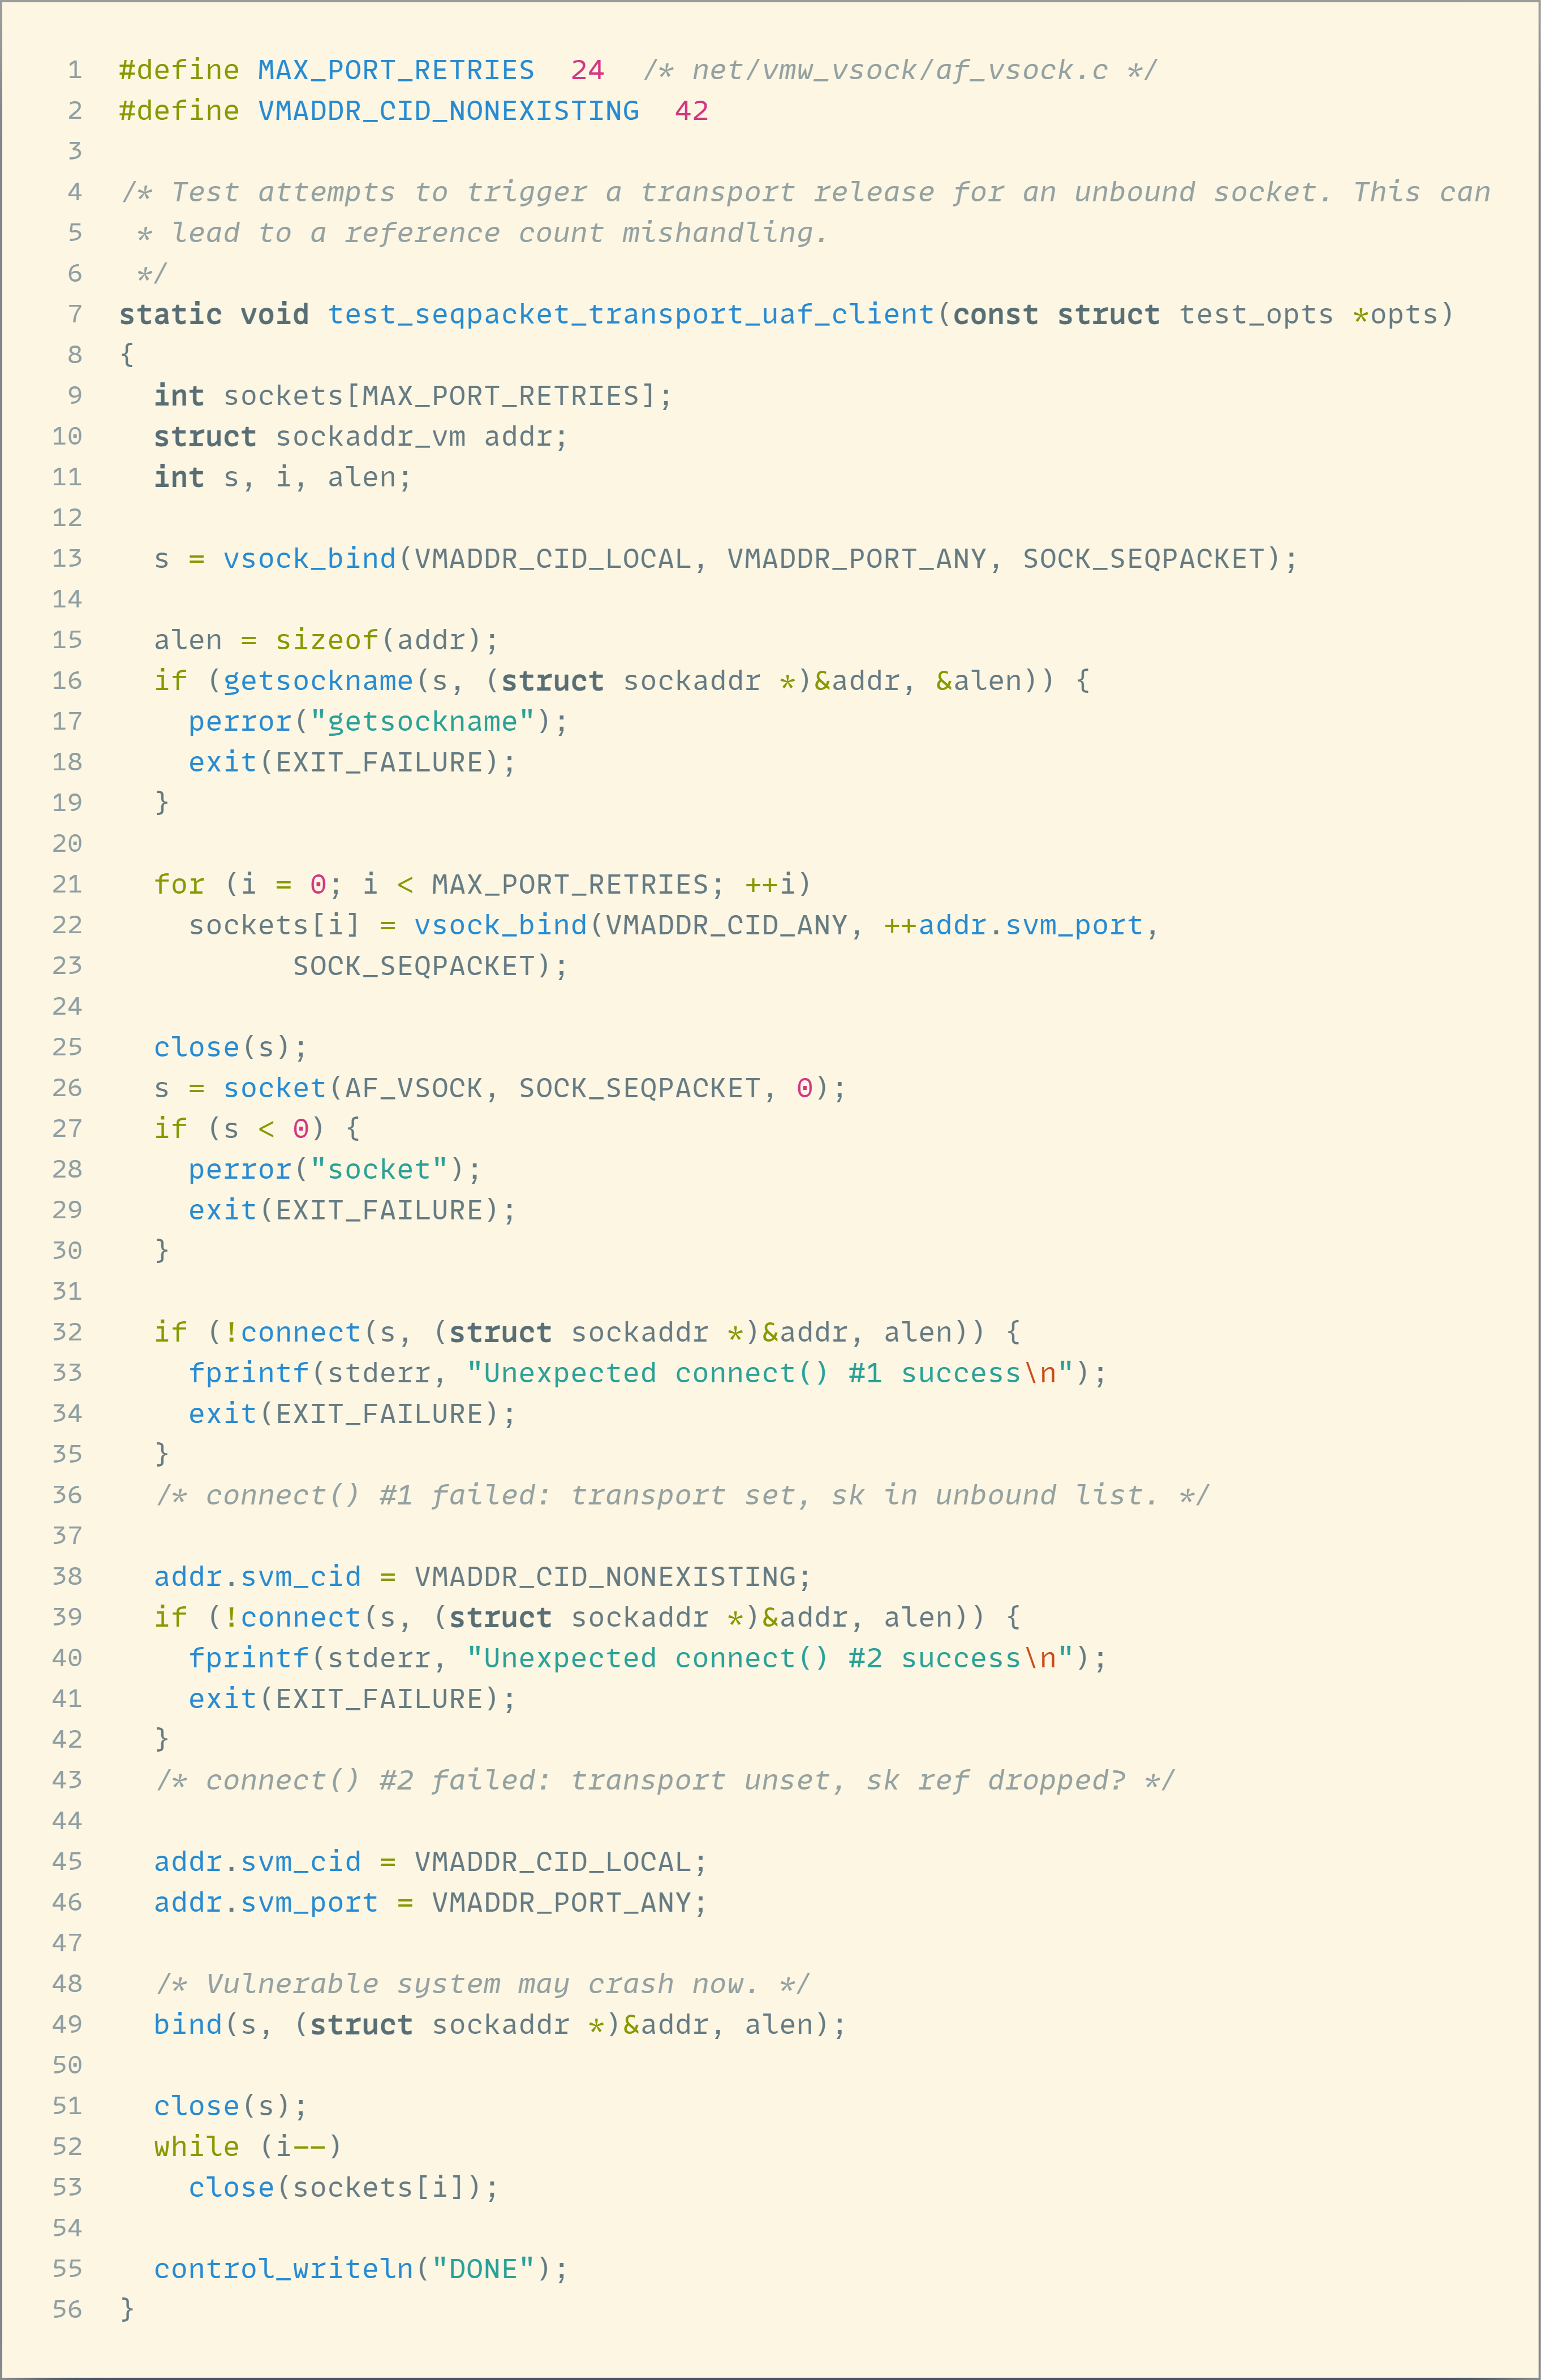
\includegraphics[scale=.14]{images/test_case.png}
    \caption{The test case provided by the maintenance developers.}
    \label{fig:test_case}
\end{figure}
\noindent The test case in question does not lead to a privilege escalation, but causes the kernel to crash on vulnerable systems. By examining it step by step, it is possible to understand what is going wrong in the reference counting mechanism associated with a vsock socket.

\subsubsection{Step-by-step analysis}
Let's look at every relevant step in the test case. Every function will be described in detail in section \ref{functions_involved}.

\begin{figure}[H]
    \centering
    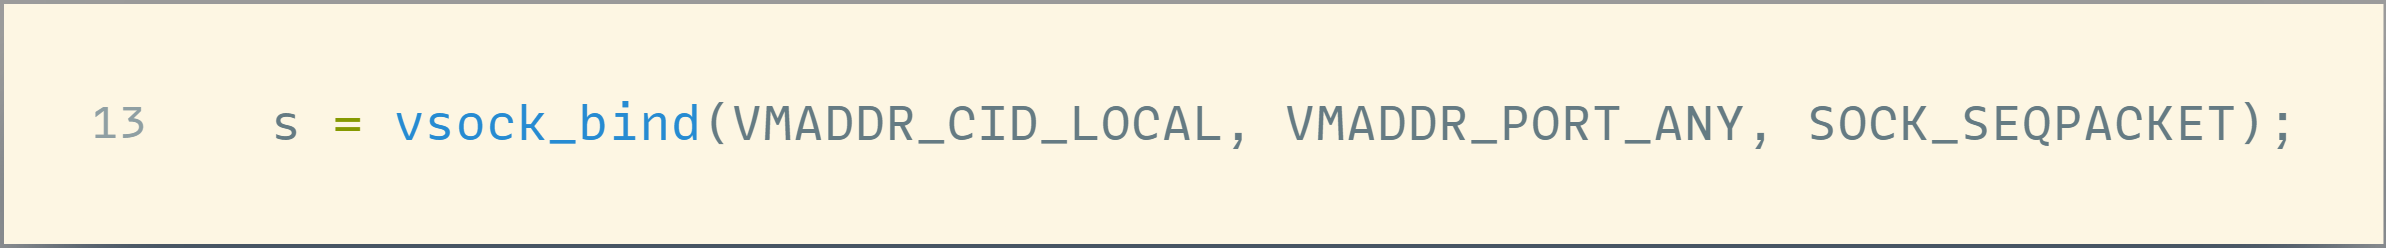
\includegraphics[scale=.14]{images/tc1.png}
    \label{fig:tc1}
\end{figure}

% TODO - continuare

\section{Functions involved}\label{functions_involved}



\section{Patches and mitigation measures}

\section{Overview of the exploit}
